\documentclass{report}
\input{preamble}
\input{macros}
\input{letterfonts}

\title{\Huge{BC Calculus - Middlesex School}\\Lab - Approximating functions by Polynomials }
\author{\huge{Ben Feuer \& Joey Casper}}
\date{}

\begin{document}

\maketitle
\newpage% or \cleardoublepage
% \pdfbookmark[<level>]{<title>}{<dest>}
\pdfbookmark[section]{\contentsname}{toc}
\tableofcontents
\pagebreak

\chapter{}

\section{Introduction}
In this lab, we approximate $ e^x $ using polynomials in order to use our approximation for $ e^x $ to approximate the integral $ \frac{1}{\sqrt{2\pi } } \int _0 ^ \frac{1}{2} e^{-x^2} $.

\section{Finding our approximation for $e^x$}
To find our approximation, we used DESMOS in which we created a polynomial $ y = 1 + ax + bx^2 + c^3 $ where we manipulated the parameters, $ a, b, c $ in order to get the best fit polynomial to $ e^x $ from -1 to 1. Through this method we found that the parameters to be a = 1, b = .5, and c = .25. 
\\
\\
Below are the steps we took in making our polynomial(adding another degree in each step):

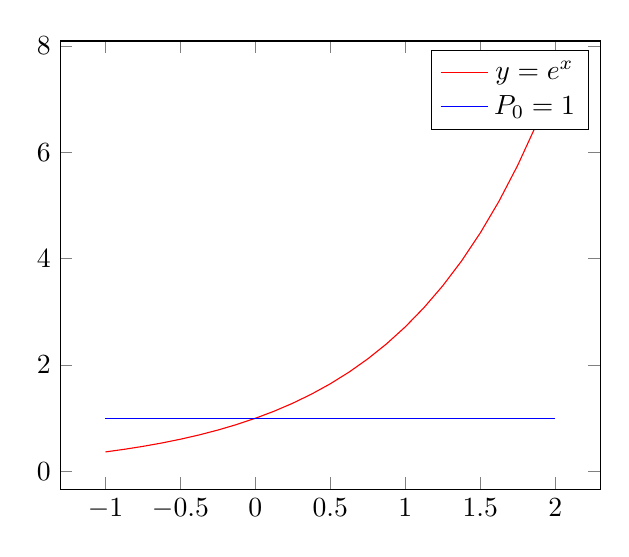
\begin{tikzpicture}
  \begin{axis}[
    domain=-1:2
    ]
    \addplot[color=red]{exp(x)};
    \addlegendentry{$y=e^x$}
    
      \addplot[color=blue]{1};
    \addlegendentry{$P_0=1$}
  \end{axis}
\end{tikzpicture}

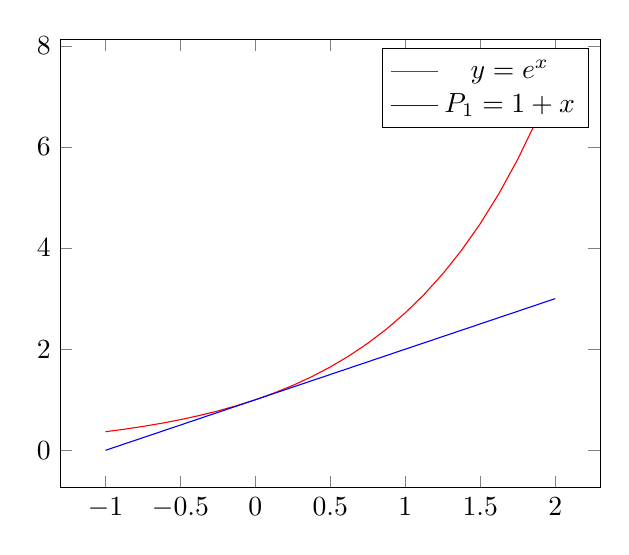
\begin{tikzpicture}
  \begin{axis}[
    domain=-1:2
    ]
    \addplot[color=red]{exp(x)};
    \addlegendentry{$y=e^x$}
    
      \addplot[color=blue]{1+x};
    \addlegendentry{$P_1=1 + x$}
  \end{axis}
\end{tikzpicture}

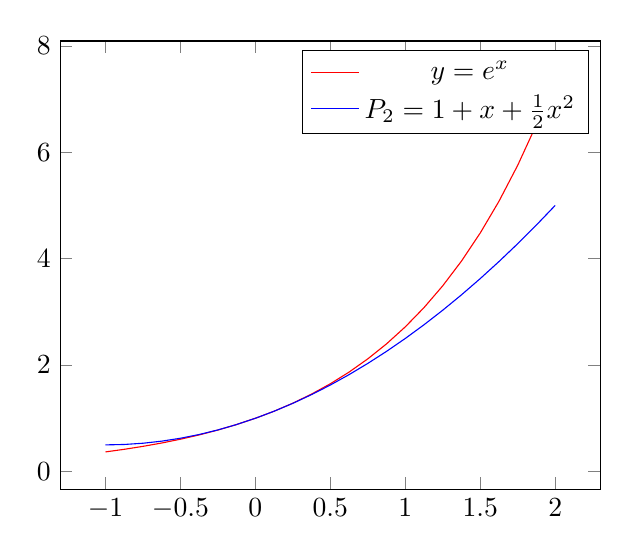
\begin{tikzpicture}
  \begin{axis}[
    domain=-1:2
    ]
    \addplot[color=red]{exp(x)};
    \addlegendentry{$y=e^x$}
    
      \addplot[color=blue]{1+x+1/2*x^2};
      \addlegendentry{$P_2=1 + x + \frac{1}{2}x^2$}
  \end{axis}
\end{tikzpicture}

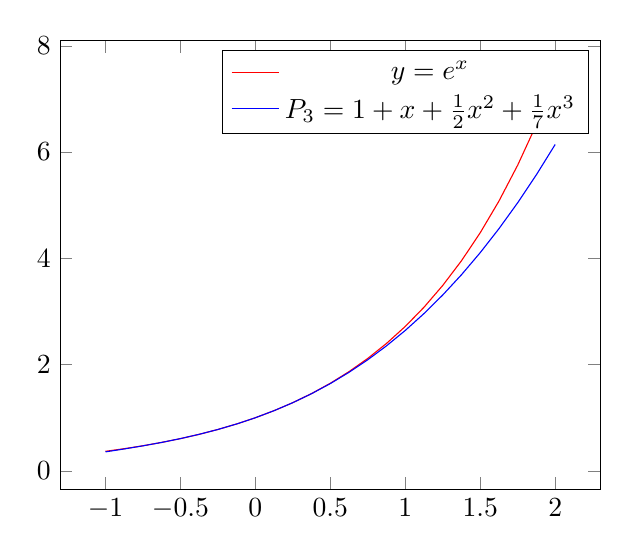
\begin{tikzpicture}
  \begin{axis}[
    domain=-1:2
    ]
    \addplot[color=red]{exp(x)};
    \addlegendentry{$y=e^x$}
    
      \addplot[color=blue]{1+x+1/2*x^2 + 1/7*x^3};
      \addlegendentry{$P_3=1 + x + \frac{1}{2}x^2 + \frac{1}{7}x^3$}
  \end{axis}
\end{tikzpicture}

As shown above, our final approximation for $e^x$ is $P_3=1 + x + \frac{1}{2}x^2 + \frac{1}{7}x^3$.

\section{Testing our approximation's accuracy}
To test our approximation of $ e^x $, we compare the function $P_3(0.5)$ with $e^{0.5}$. The difference between $P_3(0.5)$ and $e^{0.5}$ is 0.0058 with our approximation underapproximating the true value of $e^x$. This marginal underapproximation is less on the other points of the interval $ [0,0.5]$, and you can visualize this difference below where you can see how the approximation is quite accurate from about -1 to 1.


\begin{tikzpicture}
  \begin{axis}[
    domain=-2:2
    ]
      \addplot[color=blue]{exp(x) -1-x-1/2*x^2-1/7*x^3};
      \addlegendentry{$e^x - P_3$}
  \end{axis}
\end{tikzpicture}

\section{Applying this approximation to compute an integrand that has no antiderivitive}

With this approximation for $e^x$, we can now evaluate $\int _0 ^{0.5} e^{-x^2} dx $ by using $ P_3(-x^2)$. This gives us the new approximated function for $ e^{-x^2} $ which equals $ P_3(-x^2) = 1 - x^2 + \frac{1}{2}x^4 - \frac{1}{7}x^6$. With this polynomial function we can now solve for the integral which is equal to:
$$ \int _0 ^{0.5} 1 - x^2 + \frac{1}{2}x^4 - \frac{1}{7}x^6 dx = 0.461298894558  $$

This is very similar to the answer the calculator gives for the actual function(0.461281006413) as it is equal up until the fifth decimal place.

\section{Using the analytical method that is also used in finding Taylor polynomials}

\begin{itemize}
  \item $\frac{f'}{1} = 1 $
  \item $\frac{f''}{\frac{1}{2}} = 2$
  \item $\frac{f'''}{\frac{1}{7}} = 6$
\end{itemize}

% diagrams/picutre.png
\begin{figure}
  \begin{center}
    \includegraphics[width=0.95\textwidth]{figures/image.png}
  \end{center}
  \caption{Table that determines a,b, and c}
  \label{fig:}
\end{figure}



Now with these values for each degree (from 1 to 3) of the polynomial, we can now determine the cubic Taylor polynomial for the exponential function by adjusting the four coefficients so the values of the Taylor polynomial and its first three derivitives match those of $e^x$ at $x=0$.

Now we have a new value for the cubic Taylor polynomial ( $ C = \frac{1}{6} $ ). And thus now our new polynomial is $ y = 1 + x + \frac{1}{2}x^2 + \frac{1}{6}x^3 $. This new polynomial can be shown below:
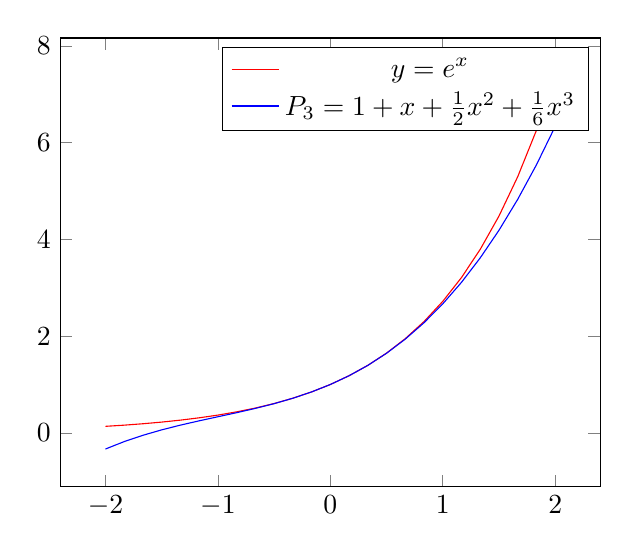
\begin{tikzpicture}
  \begin{axis}[
    domain=-2:2
    ]
    \addplot[color=red]{exp(x)};
    \addlegendentry{$y=e^x$}
    
      \addplot[color=blue]{1+x+1/2*x^2 + 1/6*x^3};
      \addlegendentry{$P_3=1 + x + \frac{1}{2}x^2 + \frac{1}{6}x^3$}
  \end{axis}
\end{tikzpicture}

where it is shown how close the two functions are to each other at $ x = 0 $

\end{document}
